%%%%%%%%%%%%%%%%%%%%%%%%%%%%%%%%%%%%%%%%%%%%%%%%%%%%%%%%%%%%%%%%%%%%%%%%%%%%%%%%
\documentclass{beamer}
%
\usepackage[italian]{babel}
\usepackage[utf8]{inputenc}
\usepackage[T1]{fontenc}

%%%% Subtitle
%\subtitle[Short Subtitle]{Full Subtitle}
%%%% Authors
%%%% Institution/Partner
%%%% Date
% Structure slides
%
%%%%%%%%%%%%%%%%%%%%%%%%%%%%%%%%%%%%%%%%%%%%%%%%%%%%%%%%%%%%%%%%%%%%%%%%%%%%%%%%
\begin{document}
\title[Lab1 - FV]{Fondamenti di Informatica A \\ Laboratorio 8 \\ Array e puntatori in C}
\author[Danilo Pianini]{Danilo Pianini\\\texttt{danilo.pianini@unibo.it} \\ \vspace{3pt} Pietro Brunetti\\\texttt{p.brunetti@unibo.it} \\ \vspace{3pt} Mirko Viroli\\\texttt{mirko.viroli@unibo.it} }
\institute[UNIBO]{\textsc{Alma Mater Studiorum}---Università di Bologna}
\date[\today]{\today}

\frame{\titlepage} 

\begin{frame}
\frametitle{Operazioni preliminari}
\begin{itemize}
 \item Accendere il computer
 \item Effettuare il log-in con le proprie credenziali istituzionali
  \begin{itemize}
    \item Normalmente sono simili a: \texttt{nome.cognome@studio.unibo.it}
  \end{itemize}
 \item Aprire Google Chrome, o altro browser
 \item Collegarsi al sito \url{http://campus.unibo.it/187209/}
 \item Scaricare il pacchetto \url{http://campus.unibo.it/187209/}
 \item Scompattare il pacchetto in una cartella a piacimento: questa sarà la vostra directory di lavoro di oggi.
\end{itemize}
\end{frame}

\begin{frame}
\frametitle{Comprensione di un esempio con puntatori}
\begin{itemize}
 \item Aprire il file \texttt{e2.c} contenente la funzione \texttt{swap} e un \texttt{main} che effettua un semplice test di essa: se ne analizzi il codice cercando di capirne il funzionamento.
 \item Prima di compilare il codice, si provi a capire quale dovrebbe essere l'output prodotto sulla console.
 \item Compilare ed eseguire. Si verifichi che l'output del programma corrisponde a quanto previsto.
\end{itemize}
\end{frame}

\begin{frame}[fragile]
\frametitle{Cosa succede? 1/7}
\begin{verbatim}
void swap(int *i1,int *i2){
   int temp=*i1;
   *i1=*i2;
   *i2=temp;
}    
int main(void){
   int a=10; // Il controllo è qui
   int b=20;
   swap(&a,&b);
}\end{verbatim}
\begin{figure}
 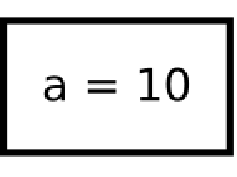
\includegraphics[width = 0.2\columnwidth]{img/1}
\end{figure}
\end{frame}

\begin{frame}[fragile]
\frametitle{Cosa succede? 2/7}
\begin{verbatim}
void swap(int *i1,int *i2){
   int temp=*i1;
   *i1=*i2;
   *i2=temp;
}    
int main(void){
   int a=10;
   int b=20; // Il controllo è qui
   swap(&a,&b);
}\end{verbatim}
\begin{figure}
 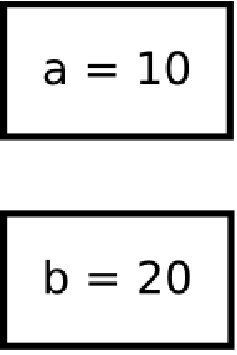
\includegraphics[width = 0.2\columnwidth]{img/2}
\end{figure}
\end{frame}

\begin{frame}[fragile]
\frametitle{Cosa succede? 3/7}
\begin{verbatim}
void swap(int *i1,int *i2){  // Il controllo è qui
   int temp=*i1;
   *i1=*i2;
   *i2=temp;
}    
int main(void){
   int a=10;
   int b=20;
   swap(&a,&b);
}\end{verbatim}
\begin{figure}
 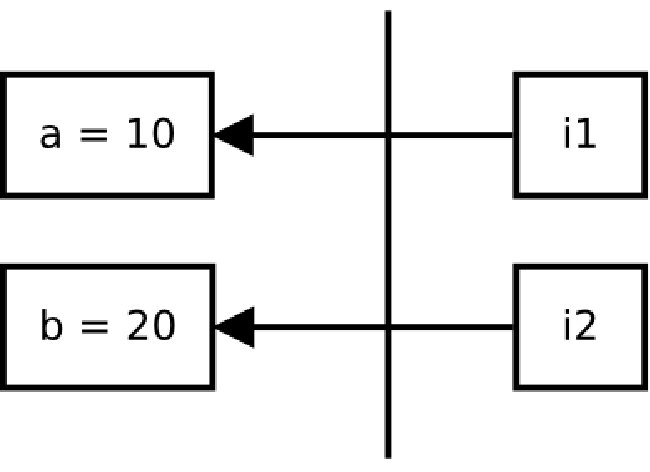
\includegraphics[width = 0.4\columnwidth]{img/3}
\end{figure}
\end{frame}

\begin{frame}[fragile]
\frametitle{Cosa succede? 4/7}
\begin{verbatim}
void swap(int *i1,int *i2){
   int temp=*i1; // Il controllo è qui
   *i1=*i2;
   *i2=temp;
}    
int main(void){
   int a=10;
   int b=20;
   swap(&a,&b);
}\end{verbatim}
\begin{figure}
 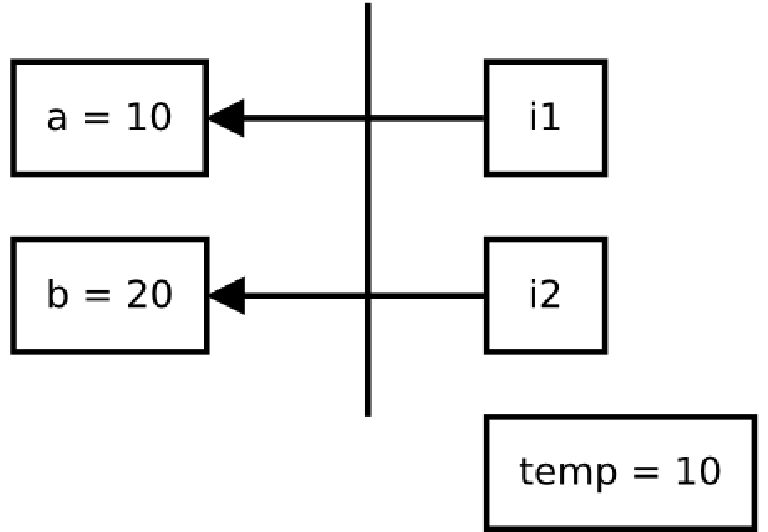
\includegraphics[width = 0.4\columnwidth]{img/4}
\end{figure}
\end{frame}

\begin{frame}[fragile]
\frametitle{Cosa succede? 5/7}
\begin{verbatim}
void swap(int *i1,int *i2){
   int temp=*i1;
   *i1=*i2; // Il controllo è qui
   *i2=temp;
}    
int main(void){
   int a=10;
   int b=20;
   swap(&a,&b);
}\end{verbatim}
\begin{figure}
 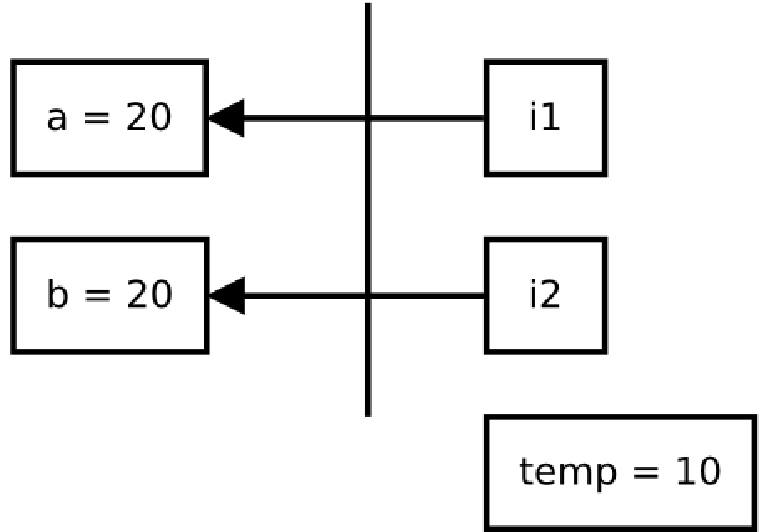
\includegraphics[width = 0.4\columnwidth]{img/5}
\end{figure}
\end{frame}

\begin{frame}[fragile]
\frametitle{Cosa succede? 6/7}
\begin{verbatim}
void swap(int *i1,int *i2){
   int temp=*i1;
   *i1=*i2;
   *i2=temp; // Il controllo è qui
}    
int main(void){
   int a=10;
   int b=20;
   swap(&a,&b);
}\end{verbatim}
\begin{figure}
 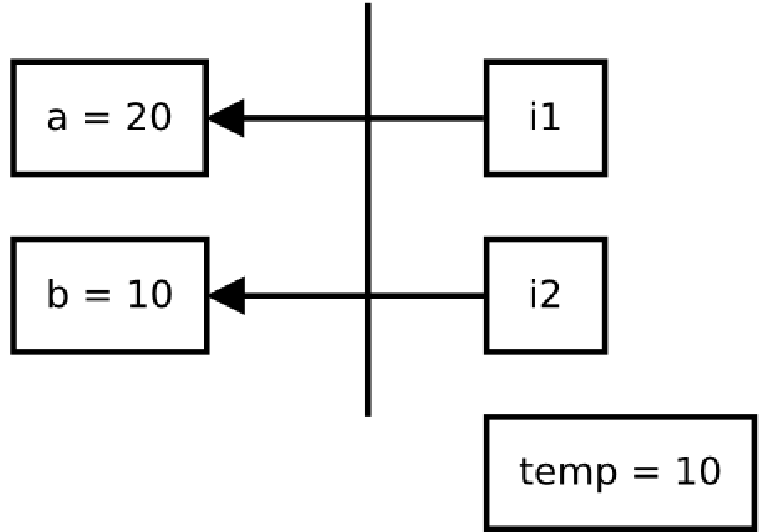
\includegraphics[width = 0.4\columnwidth]{img/6}
\end{figure}
\end{frame}

\begin{frame}[fragile]
\frametitle{Cosa succede? 7/7}
\begin{verbatim}
void swap(int *i1,int *i2){
   int temp=*i1;
   *i1=*i2;
   *i2=temp;
}    
int main(void){
   int a=10;
   int b=20;
   swap(&a,&b); // Il controllo è qui
}\end{verbatim}
\begin{figure}
 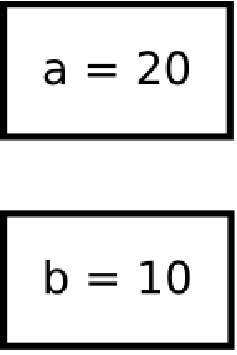
\includegraphics[width = 0.2\columnwidth]{img/7}
\end{figure}
\end{frame}

\begin{frame}
\frametitle{Modifica dell'esempio}
Si modifichi \texttt{e2.c} come segue:
\begin{itemize}
 \item Si elimini il contenuto del \texttt{main}.
 \item Si crei sullo stack (sintassi \texttt{\{10, 20, 30, 40\}}) un nuovo array di interi, contenente i valori 10, 20, 30 e 40.
 \item Si stampi il valore dei quattro elementi dell'array tramite apposita \texttt{printf}
 \item Si invochi la funzione \texttt{swap} passando come primo argomento il puntatore al primo valore dell'array e come secondo argomento il puntatore al secondo elemento dell'array (suggerimento: l'accesso all'i-esimo elemento dell'array a si effettua tramite \texttt{a[i]}, mentre il puntatore all'i-esimo elemento di a si può ottenere con \texttt{\&a[i]})
 \item Si stampi nuovamente il valore dei quattro elementi dell'array tramite apposita \texttt{printf}
 \item Si compili ed esegua: il risultato è conforme alle attese?
\end{itemize}
\end{frame}

\begin{frame}
\frametitle{\texttt{void *malloc(unsigned int size)}}
La funzione \texttt{void *malloc(unsigned int size)} consente di allocare per il programma una porzione di memoria nello heap grande \texttt{size} bytes.
\begin{itemize}
 \item Si osservi il contenuto di \texttt{create\_array.c}. Cosa fa? Una volta compreso il funzionamento, si compili e si esegua.
 \item Si modifichi \texttt{create\_array.c} affinché crei un nuovo array il cui contenuto sia numerato progressivamente (e.g. \texttt{create\_array(5)} deve tornare \texttt{\{1,2,3,4,5\}}. Si modifichi il \texttt{main} perché stampi a video l'intero contenuto dell'array con gli elementi separati da spazi, quindi vada a capo.
\end{itemize}
\end{frame}

\begin{frame}
\frametitle{Stringhe di caratteri in C}
Diversamente da Java, C non ha supporto per il tipo \texttt{String} a livello di linguaggio. In C, le Stringhe sono in realtà dei \texttt{char *} (ossia anche dei \texttt{char []}), terminati dal carattere speciale \texttt{\textbackslash{}0}.
\begin{itemize}
 \item Utilizzando anche la funzione malloc vista in precedenza, e facendo riferimento ai lucidi visti a lezione, si realizzi una funzione che concatena due stringhe, separandole con uno spazio, ossia col carattere \texttt{' '} (si noti che la concatenazione semplice è già risolta nei lucidi!)
 \item Si scriva un \texttt{main} che concateni le stringhe \textquotedbl{}ottimo\textquotedbl{} e \textquotedbl{}lavoro\textquotedbl{}. E le stampi a video. Si ricordi che è possibile stampare con \texttt{printf} un \texttt{char *} direttamente.
 \item Si scriva una funzione \texttt{char scanToLast(char *s)} che, data una stringa di lunghezza non nota, torna l'ultimo elemento. Non è consentito l'uso di \texttt{strlen}. La si testi nel \texttt{main}.
\end{itemize}
\end{frame}

\begin{frame}
\frametitle{Output negli argomenti}
I puntatori consentono di utilizzare argomenti come output: si passa un puntatore all'area in cui vogliamo il risultato, la funzione computa e scrive in quell'area il risultato, in questo modo il chiamante può accedervi. Si faccia riferimento alla slide 10 del pacchetto \texttt{06d-C-array\_puntatori2.pdf}.
\begin{itemize}
 \item Si realizzi la funzione\\ \texttt{void sum(int a, int b, int *res)} \\che dati due interi ne calcola la somma e la mette nell'area di memoria puntata da res. Si verifichi nel \texttt{main} il funzionamento.
 \item Si implementi nel file \texttt{array\_creator.c} la funzione\\ \texttt{void arrayCreator(int size, int **res)} \\che crea un array di interi lungo \texttt{size} nell'area di memoria puntata da res, utilizzando la \texttt{malloc}, quindi lo riempie con valori crescenti a partire da 0.
\end{itemize}
\end{frame}

\begin{frame}
\frametitle{Esercizi aggiuntivi}
Chi ha terminato gli esercizi di base, può dar libero sfogo alle proprie abilità svolgendo quelli aggiuntivi.
\end{frame}

\begin{frame}
\frametitle{Riconoscitori di grammatiche in C}
Si risolvano gli esercizi proposti nei file \texttt{e3.c} ed \texttt{e4.c}, sull'implementazione di un semplice riconoscitore di grammatiche e della sua versione ricorsiva.
\end{frame}

% \begin{frame}
% \frametitle{Matrici in C}
% \begin{itemize}
%  \item Si osservi il file \texttt{matr.c}. Se ne comprenda il funzionamento, e solo dopo averlo compreso si compili e si esegua.
%  \item Sulla base di matr.c, si crei un nuovo programma in \texttt{matrBorder.c}, che crea una matrice della dimensione desiderata, quindi ne resetta il bordo esterno (prima e ultima riga, prima e ultima colonna).
% \end{itemize}
% \end{frame}
% 
% \begin{frame}
% \frametitle{Output negli argomenti}
% Perché fermarsi ai puntatori a puntatore quando si possono fare puntatori a puntatori a puntatori? (e via per induzione...)
% \begin{itemize}
%  \item Si realizzi all'interno di matr.c la funzione\\ \texttt{void matrixCreator(int size, int ***res)} \\che crea una matrice quadrata di interi grande \texttt{size} nell'area di memoria puntata da res, utilizzando la \texttt{malloc}, quindi lo riempie con valori crescenti a partire da 0. Si usi nel \texttt{main} questa funzione al posto di \\ \texttt{int **matr(int size,int elem)}.
% \end{itemize}
% \end{frame}


\end{document}

